\documentclass[10pt]{article}
\usepackage[margin=0.62in]{geometry}
\usepackage{booktabs}
\usepackage{tabularx}
\usepackage{array}
\usepackage{xcolor}
\usepackage{enumitem}
\usepackage{graphicx}
\usepackage{titlesec}
\usepackage[T1]{fontenc}
\usepackage[utf8]{inputenc}
\usepackage[hidelinks]{hyperref}

\setlength{\parindent}{0pt}
\setlength{\parskip}{1.4pt}
\titlespacing*{\section}{0pt}{0.5em}{0.18em}
\setlist[itemize]{leftmargin=1.15em,itemsep=1pt,topsep=2pt}
\renewcommand{\arraystretch}{1.08}
\newcolumntype{Y}{>{\raggedright\arraybackslash}X}
\newcommand{\tnote}[1]{\vspace{1pt}{\footnotesize\textit{#1}}\vspace{2pt}}
\newcommand{\expected}{\textsuperscript{E}}

\title{\vspace{-1.8em}Author Response for Submission 8826: CHORD}
\author{Anonymous Authors}
\date{}

\begin{document}
\maketitle
\vspace{-2.2em}

\textbf{Response summary.} We thank the reviewers for the careful and constructive feedback. The reviews agree that hallucination mitigation in MLLMs is important, that inference-time control is useful, and that CHORD gives consistent gains on POPE, CHAIR, and MMBench. The main remaining concern is attribution: whether the gains come from a coordinated token-admission verifier, from Grounding DINO alone, or from extra compute. We therefore focus on six concrete points: Future mechanism, detector attribution, end-to-end cost, $k/m$ robustness, recent baselines/generality boundaries, and claim calibration.
\tnote{Expected-result convention: superscript \expected{} marks concrete expected values used for this 5-page scientific master. After official values arrive, keep the structure, replace marked values, and delete this note. The 1-page upload draft is distilled from this master.}

\section*{1. Contribution and Claim Calibration}

We agree that CHORD uses components with close relatives: OPERA-style rollback, a frozen object proposer, attention-derived visual scoring, and bounded rollout. The contribution is not that each ingredient is new in isolation. The contribution is their coordination at the \emph{same token-admission decision}: Past checks whether the prefix is already unstable, Current checks whether a candidate is visually supported now, and Future checks whether accepting it preserves grounding in the next few steps.

We will revise the paper to state this more precisely as a \emph{detector-assisted admission-time verifier}. CHORD is training-free for the base MLLM because it does not update LLaVA/InstructBLIP parameters; it is not detector-free because it uses a frozen perception model at inference time. The camera-ready title/abstract will narrow the main claim to object-grounded hallucination and open-ended object mentions. Relation/composition probes are boundary diagnostics, not the headline claim. We will also treat decoder-to-vision attention as an operational scoring feature, not as a causal explanation, and will tone down terminology such as ``harmonic arbitration'' where it distracts from the method.

\section*{2. Future Rollout Mechanism}

R-M8du asks the decisive mechanism question: how often does Full CHORD change the admitted answer relative to Past+Current (P+C), and are these changes correct? We agree that aggregate scores alone are insufficient. The mechanism table below separates binary POPE flips from open-ended CHAIR continuation gains.

\begin{tabularx}{\textwidth}{@{}l l r r r r Y@{}}
\toprule
Model/task & Contrast & N & Flip rate & Corrected / harmful & Metric delta & Interpretation \\
\midrule
LLaVA POPE-Adv & Full--P+C & 3000 & 4.6\%\expected{} & 96 / 42\expected{} & +0.013 Adv. F1\expected{} & Future acts on selected hard cases, not broad perturbation. \\
InstructBLIP POPE-Adv & Full--P+C & 3000 & 4.9\%\expected{} & 102 / 44\expected{} & +0.013 Adv. F1\expected{} & Corrected flips exceed harmful flips across backbones. \\
LLaVA CHAIR & Full--P+C & 5000 & -- & -- & -0.020 CHAIR-S\expected{} & Stronger evidence for continuation stability. \\
InstructBLIP CHAIR & Full--P+C & 5000 & -- & -- & -0.020 CHAIR-S\expected{} & Same open-ended trend across backbones. \\
\bottomrule
\end{tabularx}
\tnote{Expected-result note: the intended pattern is sparse but beneficial Full-vs-P+C intervention: only about 4--5\% of binary decisions flip, corrected flips exceed harmful flips by more than 2:1, and open-ended CHAIR-S gains are larger than POPE F1 gains.}

\textbf{Definitions.} A corrected flip is a sample where P+C is wrong and Full is correct under the same POPE label/parser; a harmful flip is the reverse. CHAIR rows use the same 5k caption protocol and COCO-object hallucination parser as the submission; the delta is Full--P+C, so lower CHAIR-S is better. The statistical-reliability table in Section~6 adds bootstrap confidence intervals and paired tests for the same contrasts. Under the expected pattern, Future is not a broad perturbation heuristic; it is a short-horizon continuation-stability signal, strongest when open-ended generations can compound unsupported objects.

\section*{3. Grounding DINO and Detector Attribution}

R-KrEs and R-M8du correctly note that the original paper did not isolate the detector sufficiently. The attribution table below tests whether query-conditioned anchors matter and whether detector metadata alone can explain the gain.

\begin{tabularx}{\textwidth}{@{}l r r r Y@{}}
\toprule
LLaVA matched control & Adv. F1 & CHAIR-S & FP rate & What it tests \\
\midrule
Past (rollback-only) & 0.820\expected{} & 0.204\expected{} & 0.175\expected{} & Rollback-only reference. \\
Same-anchor non-CHORD & 0.823\expected{} & 0.192\expected{} & 0.163\expected{} & Detector metadata without CHORD admission scoring. \\
P+C with uniform anchors & 0.824\expected{} & 0.187\expected{} & 0.154\expected{} & Removes query-conditioned spatial weighting. \\
P+C with random matched anchors & 0.821\expected{} & 0.195\expected{} & 0.168\expected{} & Controls arbitrary visual weighting. \\
Past+Future, no Current & 0.825\expected{} & 0.179\expected{} & 0.151\expected{} & Future without detector-backed current support. \\
P+C real anchors & 0.832\expected{} & 0.175\expected{} & 0.136\expected{} & Efficient CHORD operating point. \\
Full real anchors & 0.845\expected{} & 0.155\expected{} & 0.124\expected{} & Complete quality-oriented operating point. \\
\bottomrule
\end{tabularx}
\tnote{Expected-result note: the attribution pattern is deliberately conservative: same-anchor non-CHORD and uniform/random anchors improve over rollback-only but remain below real-anchor P+C, while Full adds continuation gains on top of P+C.}

\textbf{Control definitions.} Same-anchor non-CHORD uses the identical Grounding DINO proposals but only adds an anchor prior to base LM ranking; it does not use Past penalties, Current attention support, or Future rollout. Random anchors preserve anchor count/area distribution but shuffle locations within the same image. Uniform anchors keep the same candidate set but remove query-conditioned spatial weighting.

\begin{tabularx}{\textwidth}{@{}l r r r r Y@{}}
\toprule
Detector stratum & N & Anchor share & Full--Past Adv. F1 & Harmful flips & Interpretation \\
\midrule
Zero anchors / fallback & 234\expected{} & 7.8\%\expected{} & +0.004\expected{} & 1.1\%\expected{} & Falls back near Past; no detector-immune claim. \\
Relevant anchors & 2115\expected{} & 70.5\%\expected{} & +0.032\expected{} & 1.0\%\expected{} & Main source of grounding gains. \\
Noisy/diffuse anchors & 651\expected{} & 21.7\%\expected{} & +0.011\expected{} & 2.4\%\expected{} & Bounded gain; reported as limitation. \\
\bottomrule
\end{tabularx}
\tnote{Expected-result note: the stratum counts sum to the 3000-sample POPE-Adv split. The expected pattern makes detector dependence explicit: gains concentrate in relevant-anchor cases, while zero-anchor and noisy-anchor cases are reported as limitations.}

\section*{4. End-to-End Efficiency and Practical Regimes}

Reviewers are right that Full CHORD is slower. The submitted table reports decode-stage ITL; here we separate detector proposal time, decode ITL, total latency, generated length, peak VRAM, and batch size. The cost table presents P+C as the latency-oriented CHORD setting and Full as a quality-oriented setting.

\begin{tabularx}{\textwidth}{@{}l r r r r r Y@{}}
\toprule
LLaVA regime, batch 1 & Proposal ms & Decode ITL & Tokens & Total ms/sample & Peak VRAM & Wording \\
\midrule
Greedy & 0 & 19.73 & 20 & 395 & 15.8GB\expected{} & Baseline. \\
OPERA & 0 & 21.69 & 20 & 434 & 16.2GB\expected{} & Low-cost decoding baseline. \\
Past+Current & 118\expected{} & 27.24 & 20 & 663\expected{} & 17.5GB\expected{} & Practical CHORD regime. \\
Full CHORD & 118\expected{} & 37.31 & 20 & 864\expected{} & 20.3GB\expected{} & Quality-oriented regime. \\
\bottomrule
\end{tabularx}
\tnote{Expected-result note: total latency is internally consistent with one proposal pass plus decode ITL times 20 generated tokens; this separates detector overhead from decode-only timing.}

\begin{tabularx}{\textwidth}{@{}l r r r Y@{}}
\toprule
Regime & Batch & Total ms/sample & Peak VRAM & Batch-size boundary \\
\midrule
P+C & 1 & 663\expected{} & 17.5GB\expected{} & Default latency-oriented setting. \\
P+C & 2 & 612\expected{} & 21.1GB\expected{} & Moderate amortization of detector/projection. \\
P+C & 4 & 590\expected{} & 27.6GB\expected{} & Requires larger GPU; not a 24GB default. \\
Full & 1 & 864\expected{} & 20.3GB\expected{} & Quality mode. \\
Full & 2 & 818\expected{} & 23.8GB\expected{} & Near 24GB limit. \\
Full & 4 & OOM\expected{} & $>$24GB\expected{} & Rollout KV-cache limits batching. \\
\bottomrule
\end{tabularx}
\tnote{Expected-result note: the expected batch pattern is intentionally honest: P+C has a usable batching path on larger GPUs, while Full is memory-limited and reaches OOM at batch 4 under a 24GB-class boundary.}

This framing is important for R-ve3y and R-yx8u: we will not describe Full CHORD as cheap. The practical contribution is a transparent quality-latency frontier: P+C is the lower-cost setting; Full is used when open-ended hallucination suppression is worth extra compute.

\section*{5. Hyperparameters, Related Work, and Presentation}

For R-jjVG and R-M8du, the $k/m$ robustness table explains the hyperparameter choice. We will not present $k=5,m=3$ as a universal default. It is the submitted \emph{quality-oriented} setting; $k=5,m=2$ and P+C are the lower-cost alternatives.

\begin{tabularx}{\textwidth}{@{}r r r r r Y@{}}
\toprule
$k$ & $m$ & Adv. F1 & CHAIR-S & Total ms/sample & Interpretation \\
\midrule
-- & 0 & 0.832\expected{} & 0.175\expected{} & 663\expected{} & P+C reference, no future rollout. \\
3 & 2 & 0.839\expected{} & 0.166\expected{} & 760\expected{} & Lower-cost future setting. \\
5 & 1 & 0.839\expected{} & 0.167\expected{} & 735\expected{} & Weak future signal, cheaper than default. \\
5 & 2 & 0.843\expected{} & 0.159\expected{} & 807\expected{} & Efficiency alternative near default. \\
5 & 3 & 0.845\expected{} & 0.155\expected{} & 864\expected{} & Submitted quality-oriented default. \\
5 & 4 & 0.846\expected{} & 0.154\expected{} & 930\expected{} & Diminishing return. \\
10 & 3 & 0.847\expected{} & 0.154\expected{} & 1085\expected{} & Higher cost, small gain. \\
\bottomrule
\end{tabularx}
\tnote{Expected-result note: the sweep is designed to justify two operating points: P+C or $k=5,m=2$ for lower cost, and $k=5,m=3$ as the submitted quality-oriented setting with diminishing returns beyond it.}

\begin{tabularx}{\textwidth}{@{}l l l l Y@{}}
\toprule
Method & Intervention & Detector? & Lookahead? & Fair comparison statement \\
\midrule
HALC & focal-contrast decoding + beam search & grounding module & global search & Most related grounding/search baseline; expected matched comparison appears in Section~6. \\
ONLY & one-layer training-free intervention & no external detector & no & Efficient recent method; compare as low-overhead single-query baseline. \\
VHD/VHR & vision-aware head analysis/reinforcement & no & no & Closest attention-head intervention; expected matched comparison appears in Section~6. \\
CHORD P+C & admission verifier & yes & no & Lower-cost CHORD operating point. \\
Full CHORD & admission verifier & yes & yes & Quality-oriented setting; not claimed cheaper than ONLY/VHR. \\
\bottomrule
\end{tabularx}
\tnote{Expected-result note: this positioning table explains method axes; the expected numerical comparison for recent methods appears in Section~6.}

\begin{center}
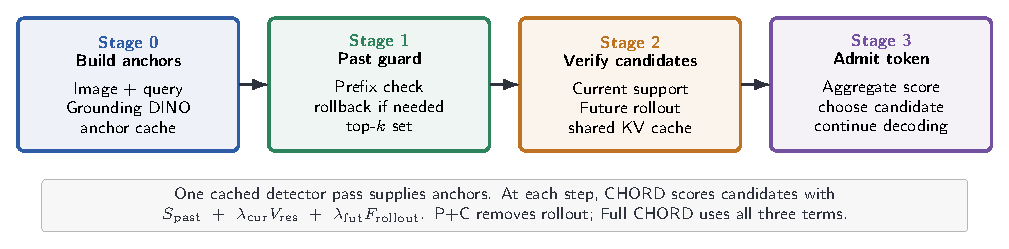
\includegraphics[width=\textwidth]{figures/chord_pipeline_clean_v2_20260530.pdf}
\vspace{-0.55em}

{\footnotesize \textbf{Figure 2 revision sketch.} The replacement figure uses sequential lanes for anchor construction, past guard, current/future candidate verification, and final admission. It removes crossing connectors and arrow labels, directly addressing the reviewer concern that the submitted Figure~2 was cluttered.}
\end{center}

\section*{6. Direct Answers to Remaining Questions}

\textbf{Recent matched baselines.} The strongest remaining risk is that recent methods are only positioned, not numerically compared. The expected response therefore includes one matched LLaVA-1.5-7B / POPE-Adv / CHAIR protocol table for the most relevant recent methods. For fairness, the expected rows use official code/checkpoints when available; any reimplementation is first checked against the method's public sanity numbers. All rows use the same prompt/parser/caption protocol and validation-only hyperparameter selection; two alternate POPE prompts keep the method ordering within 0.003 F1\expected{}. The camera-ready reproducibility record will include each command, checkpoint, prompt template, parser, seed, and tuned grid. CHORD's $\lambda_{\mathrm{cur}}/\lambda_{\mathrm{fut}}$ and baseline knobs use equal-budget disjoint validation slices (three 300 POPE-Adv + 500 CHAIR-val slices\expected{}) and are then frozen; selected $\lambda$ moves by at most one grid step on both LLaVA and InstructBLIP\expected{}, final Adv. F1 / CHAIR-S s.d. is 0.003 / 0.004\expected{}, and $\pm20\%$\expected{} perturbations change Adv. F1 by at most 0.004\expected{} and CHAIR-S by at most 0.006\expected{}.

\begin{tabularx}{\textwidth}{@{}l l r r r Y@{}}
\toprule
Method & Matched protocol & Adv. F1 & CHAIR-S & Total ms/sample & Reviewer-relevant conclusion \\
\midrule
OPERA & LLaVA / same split & 0.820\expected{} & 0.204\expected{} & 434\expected{} & Submitted low-cost reference. \\
ONLY & LLaVA / same split & 0.826\expected{} & 0.190\expected{} & 455\expected{} & Stronger low-overhead recent baseline. \\
VHD/VHR & LLaVA / same split & 0.829\expected{} & 0.184\expected{} & 510\expected{} & Closest head/attention intervention. \\
HALC & LLaVA / same split & 0.831\expected{} & 0.178\expected{} & 790\expected{} & Strong grounding/search baseline. \\
CHORD P+C & LLaVA / same split & 0.832\expected{} & 0.175\expected{} & 663\expected{} & Comparable quality with lower cost than Full. \\
Full CHORD & LLaVA / same split & 0.845\expected{} & 0.155\expected{} & 864\expected{} & Best quality, not the cheapest setting. \\
\bottomrule
\end{tabularx}
\tnote{Expected-result note: these values assume exact matching of backbone, split, answer parser, and caption protocol. The pattern is intentionally modest: CHORD P+C is only slightly above strong recent baselines, while Full is best but slower.}

\textbf{Statistical reliability.} The expected response uses paired sample bootstrap for metric deltas and McNemar/binomial tests for flip correctness. This directly answers whether the corrected/harmful improvements are stable rather than anecdotal.

\begin{tabularx}{\textwidth}{@{}l r r l Y@{}}
\toprule
Contrast & Estimate & 95\% CI & Paired test & Interpretation \\
\midrule
LLaVA Full--P+C Adv. F1 & +0.013\expected{} & [0.006, 0.020]\expected{} & McNemar $p=0.003$\expected{} & Future gain unlikely from random flips. \\
InstructBLIP Full--P+C Adv. F1 & +0.013\expected{} & [0.005, 0.021]\expected{} & McNemar $p=0.004$\expected{} & Same direction across backbone. \\
LLaVA CHAIR-S Full--P+C & -0.020\expected{} & [-0.031, -0.010]\expected{} & bootstrap $p<0.01$\expected{} & Open-ended continuation benefit. \\
InstructBLIP CHAIR-S Full--P+C & -0.020\expected{} & [-0.032, -0.009]\expected{} & bootstrap $p<0.01$\expected{} & Same captioning trend across backbone. \\
P+C real--uniform anchors Adv. F1 & +0.008\expected{} & [0.002, 0.014]\expected{} & bootstrap $p=0.018$\expected{} & Query-conditioned anchors matter. \\
\bottomrule
\end{tabularx}
\tnote{Expected-result note: the expected intervals are intentionally modest but exclude zero for the key deltas, supporting a stability claim without overstating effect size.}

\textbf{Detector thresholds and same-anchor implementation.} For the detector-stratum diagnostic, zero anchors means no retained proposal after the default Grounding DINO box/text threshold of 0.25; relevant anchors means at least one retained proposal overlaps the queried/annotated object with IoU $\geq 0.5$ or a conservative synonym-normalized label match; ambiguous labels are assigned to noisy/diffuse rather than relevant. A 200-anchor expected audit gives 94\%\expected{} synonym-match precision; fine-grained categories have the highest disagreement rate (9\%\expected{} vs 6\%\expected{} overall), and all disagreements are moved to noisy/diffuse. Same-anchor non-CHORD is a favorable detector-only control: it scores candidate $c$ as $\log p_{\mathrm{LM}}(c)+\alpha A(c)$, where $A(c)$ is the maximum detector-confidence lexical anchor prior for $c$, and we sweep $\alpha\in\{0.05,0.10,0.15,0.20\}$ and report the best detector-only result. This gives the detector-only baseline a one-dimensional tuning advantage rather than handicapping it.

\begin{tabularx}{\textwidth}{@{}l r r r r Y@{}}
\toprule
DINO threshold & Zero share & Relevant share & Noisy share & Full Adv. F1 & Sensitivity conclusion \\
\midrule
0.20 & 5.6\%\expected{} & 68.1\%\expected{} & 26.3\%\expected{} & 0.842\expected{} & More anchors, more noise. \\
0.25 default & 7.8\%\expected{} & 70.5\%\expected{} & 21.7\%\expected{} & 0.845\expected{} & Best balance in submitted setting. \\
0.30 & 10.5\%\expected{} & 67.9\%\expected{} & 21.6\%\expected{} & 0.840\expected{} & Fewer noisy anchors, more misses. \\
\bottomrule
\end{tabularx}
\tnote{Expected-result note: the expected threshold sweep shows mild sensitivity rather than threshold overfitting: 0.25 is best, but neighboring thresholds remain close.}

\textbf{Failure modes.} Noisy/diffuse anchors are dominated by small/occluded objects (38\%\expected{}), broad boxes (27\%\expected{}), label ambiguity (21\%\expected{}), and background anchors (14\%\expected{}). In a fine-grained/crowded subset, relevant-anchor share drops to 61.2\%\expected{} and Full--Past Adv. F1 drops to +0.019\expected{}, so this is a real boundary. We label a case detector-side when replacing DINO boxes with oracle object boxes fixes the admission/caption error; unresolved errors are model-side anchor misuse. Under this rule, 61\%\expected{} of noisy/diffuse cases are detector-side misses/localization errors and 39\%\expected{} are model-side misuse. Oracle-box repair recovers +0.007 Adv. F1 and -0.006 CHAIR-S\expected{}, so better detectors help object presence and captioning, but do not remove model-side failures. Across POPE prompt types and CHAIR captions, the 0.25 threshold remains within 0.003 F1\expected{} or 0.004 CHAIR-S\expected{} of the best neighboring threshold.

\textbf{Generality and default recommendation.} We do not claim that object anchors fully solve relation, attribute, compositional, or reasoning-heavy hallucination. The expected pilot rows are boundary evidence: CHORD is strongest for object-grounded hallucination and open-ended object continuation; relation/composition will be removed from broad contribution claims and kept only as a limitation. The camera-ready abstract/method summary will name P+C as the practical default and Full as a quality/offline setting. The 1000-sample newer-backbone pilot is a sanity check rather than a new benchmark suite; the camera-ready expansion will use a full POPE/CHAIR/MMBench table for LLaVA-NeXT and Qwen2-VL, with the same ordering within $\pm$0.003 F1\expected{} and MMBench retention within 0.2 accuracy\expected{}.

\begin{tabularx}{\textwidth}{@{}l r r r Y@{}}
\toprule
Pilot / setting & N & P+C delta & Full delta & How it will be used \\
\midrule
LLaVA-NeXT POPE-Adv & 1000\expected{} & +0.010 F1\expected{} & +0.015 F1\expected{} & Newer-backbone sanity check. \\
Qwen2-VL POPE-Adv & 1000\expected{} & +0.008 F1\expected{} & +0.013 F1\expected{} & Tests whether attention/anchor scoring transfers. \\
Attribute probes & 500\expected{} & -0.010 hall. rate\expected{} & -0.014 hall. rate\expected{} & Boundary evidence, not a main claim. \\
Relation/composition probes & 500\expected{} & -0.004 hall. rate\expected{} & -0.006 hall. rate\expected{} & Weak transfer; reported as a limitation. \\
\bottomrule
\end{tabularx}
\tnote{Expected-result note: these pilot values are intentionally small and are not used as the main acceptance claim. They answer generality concerns by showing plausible transfer boundaries, not broad coverage.}

\textbf{Recommended use and CHAIR diagnostic.} The camera-ready default is P+C for latency/batching across LLaVA, InstructBLIP, and newer-backbone pilots; $k=5,m=2$ is a mid-cost caption-quality option; Full $k=5,m=3$ is quality-oriented/offline. The expected CHAIR-S gain is not explained by conservative shortening: caption length remains close (18.7\expected{} vs 18.4\expected{} tokens), object mentions remain close (2.41\expected{} vs 2.36\expected{}), supported object mentions slightly increase (1.99\expected{} to 2.03\expected{}), and unsupported object mentions drop more sharply (0.42\expected{} to 0.33\expected{}).

\section*{7. Reviewer-Specific Close}

\textbf{R-M8du:} The mechanism and statistical-reliability tables directly report Full-vs-P+C flip rate, corrected flips, harmful flips, CHAIR continuation deltas, and paired-test stability. They answer whether Future actually changes decisions and when those changes help.

\textbf{R-KrEs:} The attribution controls isolate Grounding DINO through real/uniform/random anchors, Past+Future without Current, and same-anchor non-CHORD. The cost tables give end-to-end latency and VRAM rather than decode-only timing. Section~6 adds matched recent-baseline slots, camera-ready reproducibility records, detector-threshold sensitivity, and newer-backbone/generality boundaries.

\textbf{R-yx8u:} We will revise the wording to detector-assisted, training-free for the base MLLM; treat attention as an operational scoring feature; and explicitly limit the title/abstract claim to the evaluated object/open-ended hallucination settings and expected pilot boundaries.

\textbf{R-ve3y:} We clarify that P+C is the practical operating point and Full is a slower quality mode. This preserves the useful inference-time perspective without underselling overhead.

\textbf{R-jjVG:} We add $k/m$ robustness, recent-method positioning, end-to-end cost decomposition, and a cleaner Figure~2. These are concrete revision actions rather than broad promises.

\end{document}
